\documentclass[12pt]{article}
   \usepackage{amsmath}
   \usepackage{graphicx}
\begin{document}
       
\section{Server-Side protocol}
      GSN provides several HTTP request handlers that can be used to request data about sensors. In SmartD, the main requests are received by the the /gsn (gsn.http.ControllerServlet). In SmartD several request handlers have been provided. Each of these request handlers implements the gsn.http.RequestHandler interface. Each request from the clients has a REQUEST parameter (e.g., http://server/gsn?REQUEST=type) where type is an integer. Here are the list of the parameters and the Constant representing them in SmartD.
      
      
\begin{itemize}
  \item \texttt{118, REQUEST\_SMARTD}
  \item \texttt{119, REQUEST\_SMARTD\_QUESTION}
  \item \texttt{120, REQUEST\_SMARTD\_SIMILARITY}
  \item \texttt{121, REQUEST\_SMARTD\_QUESTION\_SELECTION}
  \item \texttt{122, REQUEST\_SMARTD\_NEIGHBOR\_NUM\_EVALUATION}
  \item \texttt{123, REQUEST\_SMARTD\_QUESTION\_NUM\_EVALUATION}
  \item \texttt{124, REQUEST\_SMARTD\_VALUE\_DISTRIBUTION}
\end{itemize}

\vspace{1cm}

\texttt{REQUEST\_SMARTD (http://localhost:22001/gsn?REQUEST=118\&name=electric\_data)}

\vspace{0.5cm}

This request is handled by the class gsn.vsensor.http.SmartDChartHandler. This servlet executes a query over the GSN's internal table and presents the results in the form of the stream elements. This request needs the following parameters: 

\begin{itemize}
  \item ids : individuals or groups of customers. The value can also be set to "all".
  \item startTime
  \item endTime
  \item interval: time interval
  \item intervalAggregation: min,max,sum or avg
  \item normalization: true or false
  \item aggregation: min,max,sum or avg
\end{itemize}
      
Example:  \\
  
http://localhost:22001/gsn?REQUEST=118\&name=electric\_data\&ids=1002,1018
\&startTime=2009-07-19T20:00\&endTime=2009-07-19T23:00
\&interval=30 \\ \&intervalAggregation=max
\&normalization=false\&aggregation=avg\\

Result: Figure 1.

\begin{figure}[ht!]
		\centering
			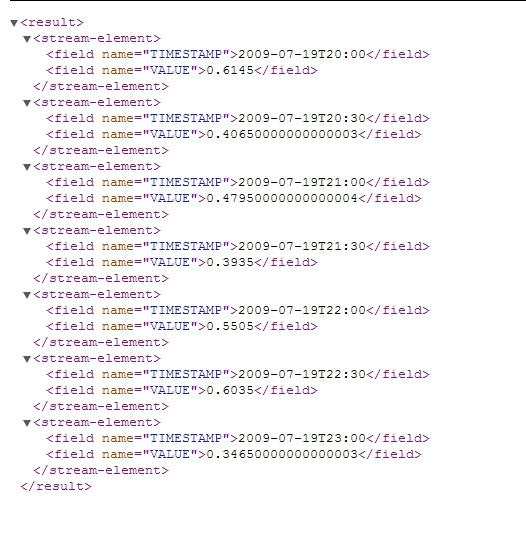
\includegraphics{REQUEST_SMARTD.JPG}
		\caption{Example}
\end{figure}

\vspace{1cm}

\texttt{REQUEST\_SMARTD\_QUESTION (http://localhost:22001/gsn?REQUEST=119)}

\vspace{0.5cm}

This request is handled by the class gsn.vsensor.http.SmartDQuestionHandler. This servlet executes a query over the GSN's internal tables containing the questions and the answer options to closed questions. This request presents the results in the form of the stream elements. This request needs the following parameter: 

\begin{itemize}
  \item question : individual question. The value can also be set to "all".
\end{itemize}
      
Example:  \\
  
http://localhost:22001/gsn?REQUEST=119\&question=8\\

Result: Figure 2.

\begin{figure}[ht!]
		\centering
			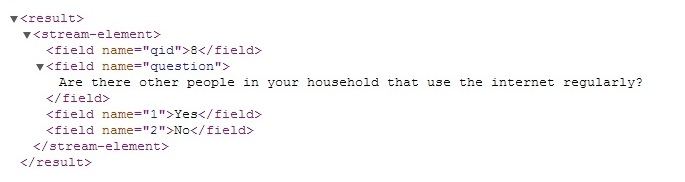
\includegraphics{REQUEST_SMARTD_QUESTION.JPG}
		\caption{Example}
\end{figure}



\vspace{1cm}

\texttt{REQUEST\_SMARTD\_SIMILARITY (http://localhost:22001/gsn?REQUEST=120)}

\vspace{0.5cm}

This request is handled by the class gsn.vsensor.http.SmartDSimilarityHandler. This servlet executes a query over the GSN's internal table and returns the average of daily energy consumption of the similar customers in the form of the stream elements. This request needs the following parameter: 

\begin{itemize}
  \item questions : group of questions and answers. 
\end{itemize}
      
Example:  \\
  
http://localhost:22001/gsn?REQUEST=120\&questions=1,1;60,2;5,1;3,2;34,1\\

Result: Figure 3.

\begin{figure}
		\centering
			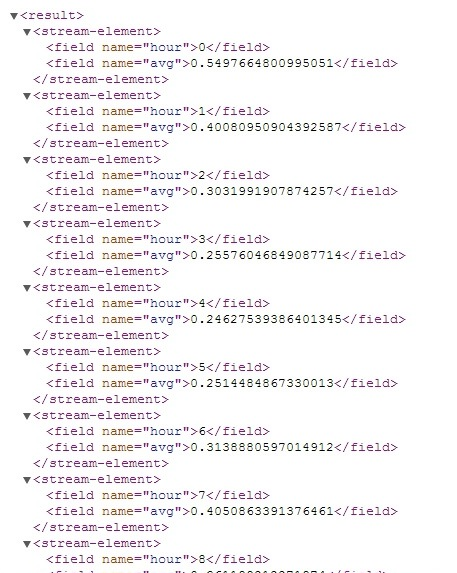
\includegraphics{REQUEST_SMARTD_SIMILARITY.JPG}
		\caption{Example}
\end{figure}


\vspace{1cm}

\texttt{REQUEST\_SMARTD\_QUESTION\_SELECTION (http://localhost:22001/gsn?REQUEST=121)}

\vspace{0.5cm}

This request is handled by the class gsn.vsensor.http.SmartDQuestionSelection. This servlet executes a query over the GSN's internal tables and returns top 5 ranked question ids in the form of the stream elements. This request needs the following parameters: 

\begin{itemize}
  \item day : sunday,monday,tuesday,wednesday,thursday,friday,saturday,weekdays or weekend.
  \item season : winter,spring,summer,autumn.
\end{itemize}
      
Example:  \\
  
http://localhost:22001/gsn?REQUEST=121\&day=weekdays\&season=winte\\

Result: Figure 4.

\begin{figure}
		\centering
			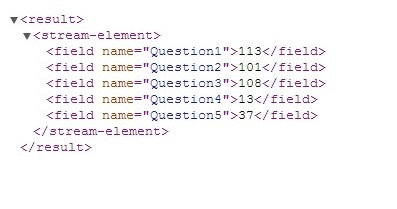
\includegraphics{REQUEST_SMARTD_QUESTION_SELECTION.JPG}
		\caption{Example}
\end{figure}


\vspace{1cm}

\texttt{REQUEST\_SMARTD\_NEIGHBOR\_NUM\_EVALUATION (http://localhost:22001/gsn?REQUEST=122)}

\vspace{0.5cm}

This request is handled by the class gsn.vsensor.http.SmartDNeighborNumEvaluation.  This request needs the following parameter: 

\begin{itemize}
  \item season : all,winter,spring,summer,autumn.
  \item neighborNum 
  \item questionNum
\end{itemize}
      
Example:  \\
  
http://localhost:22001/gsn?REQUEST=122\&neighborNum=20\&questionNum=10\\

Result: Figure 5.

\begin{figure}
		\centering
			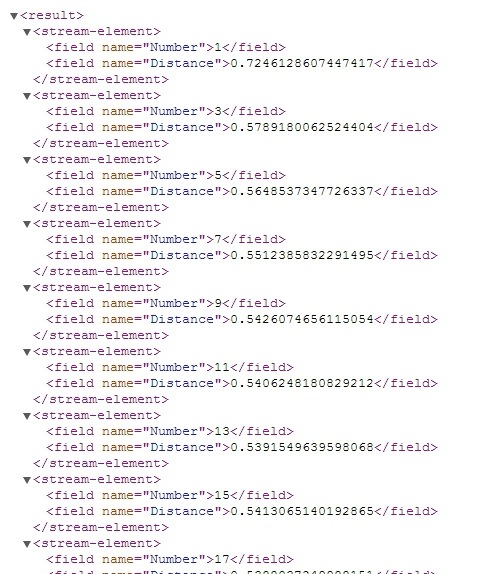
\includegraphics{REQUEST_SMARTD_NEIGHBOR_NUM_EVALUATION.JPG}
		\caption{Example}
\end{figure}


\vspace{1cm}

\texttt{REQUEST\_SMARTD\_QUESTION\_NUM\_EVALUATION (http://localhost:22001/gsn?REQUEST=123)}

\vspace{0.5cm}

This request is handled by the class gsn.vsensor.http.SmartDQuestionNumEvaluaton.  This request needs the following parameter: 

\begin{itemize}
  \item season : all,winter,spring,summer,autumn.
  \item neighborNum 
  \item questionNum
\end{itemize}
      
Example:  \\
  
http://localhost:22001/gsn?REQUEST=123\&neighborNum=20\&questionNum=10\\

Result: Figure 6.

\begin{figure}
		\centering
			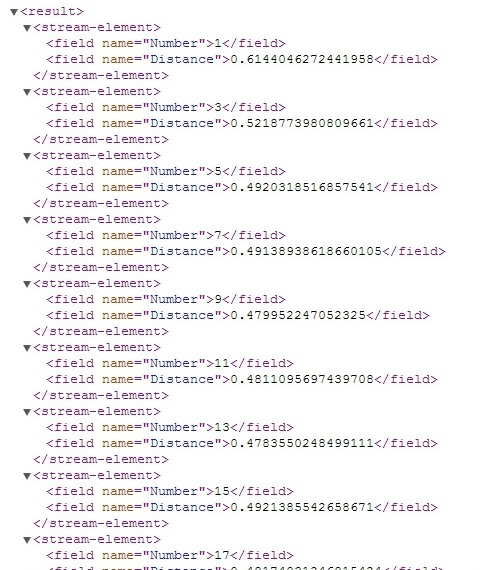
\includegraphics{REQUEST_SMARTD_QUESTION_NUM_EVALUATION.JPG}
		\caption{Example}
\end{figure}

\vspace{1cm}

\texttt{REQUEST\_SMARTD\_VALUE\_DISTRIBUTION (http://localhost:22001/gsn?REQUEST=124)}

\vspace{0.5cm}

This request is handled by the class gsn.vsensor.http.SmartDValueDistribution.  This request needs the following parameter: 

\begin{itemize}
  \item startTime 
  \item endTime
  \item bin : binSize,binNum
  \item binInput 
  \item id
\end{itemize}
      
Example:  \\
  
http://localhost:22001/gsn?REQUEST=124\&startTime=2009-07-19T01:00\&endTime=2009-07-19T23:00\&bin=binSize\&binInput=0.2\&id=1002\\

Result: Figure 7.

\begin{figure}
		\centering
			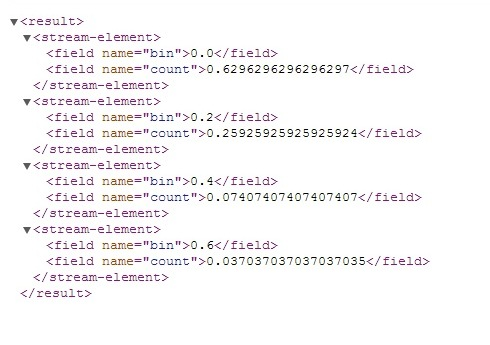
\includegraphics{REQUEST_SMARTD_VALUE_DISTRIBUTION.JPG}
		\caption{Example}
\end{figure}
      
      
\end{document}
       
    
      